\section{KẾ HOẠCH PHÁT TRIỂN}

Để đảm bảo tiến độ và chất lượng của phần mềm quản lý đặt món nhà hàng, kế hoạch phát triển được xây dựng chi tiết, phân chia thành các giai đoạn rõ ràng cho từng chức năng chính. Kế hoạch này được thể hiện qua các biểu đồ Gantt, mô tả thời gian thực hiện và các mốc quan trọng trong quá trình phát triển. Chi tiết kế hoạch có thể được xem tại: \url{https://byvn.net/fze2}.

\begin{figure}[H]
    \centering
    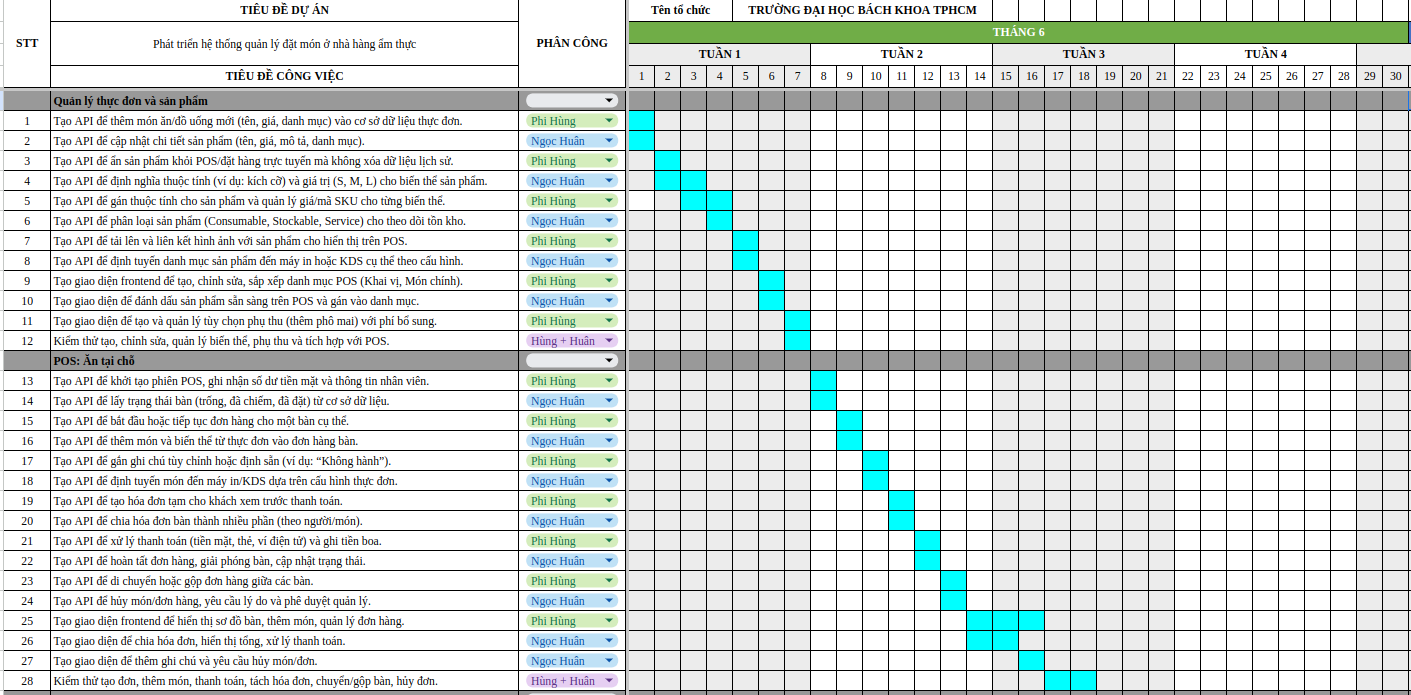
\includegraphics[width=\linewidth]{Images/gantt_1}
    \vspace{0.5cm}
    \caption{Biểu đồ Gantt cho các chức năng Quản lý thực đơn - sản phẩm và Hệ thống POS Ăn tại chỗ}
    \label{fig:gantt_menu_pos}
\end{figure}

\begin{figure}[H]
    \centering
    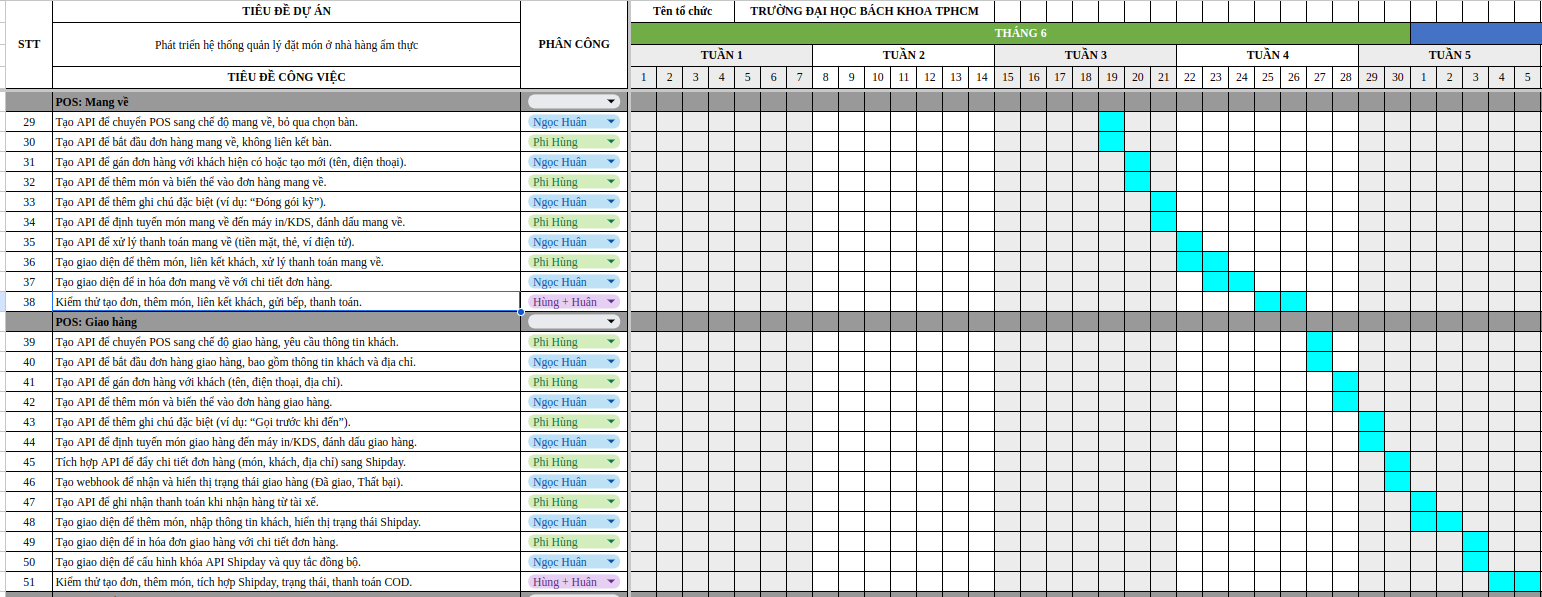
\includegraphics[width=\linewidth]{Images/gantt_2}
    \vspace{0.5cm}
    \caption{Biểu đồ Gantt cho các chức năng Hệ thống POS Mang về và Giao hàng}
    \label{fig:gantt_takeaway_delivery}
\end{figure}

\begin{figure}[H]
    \centering
    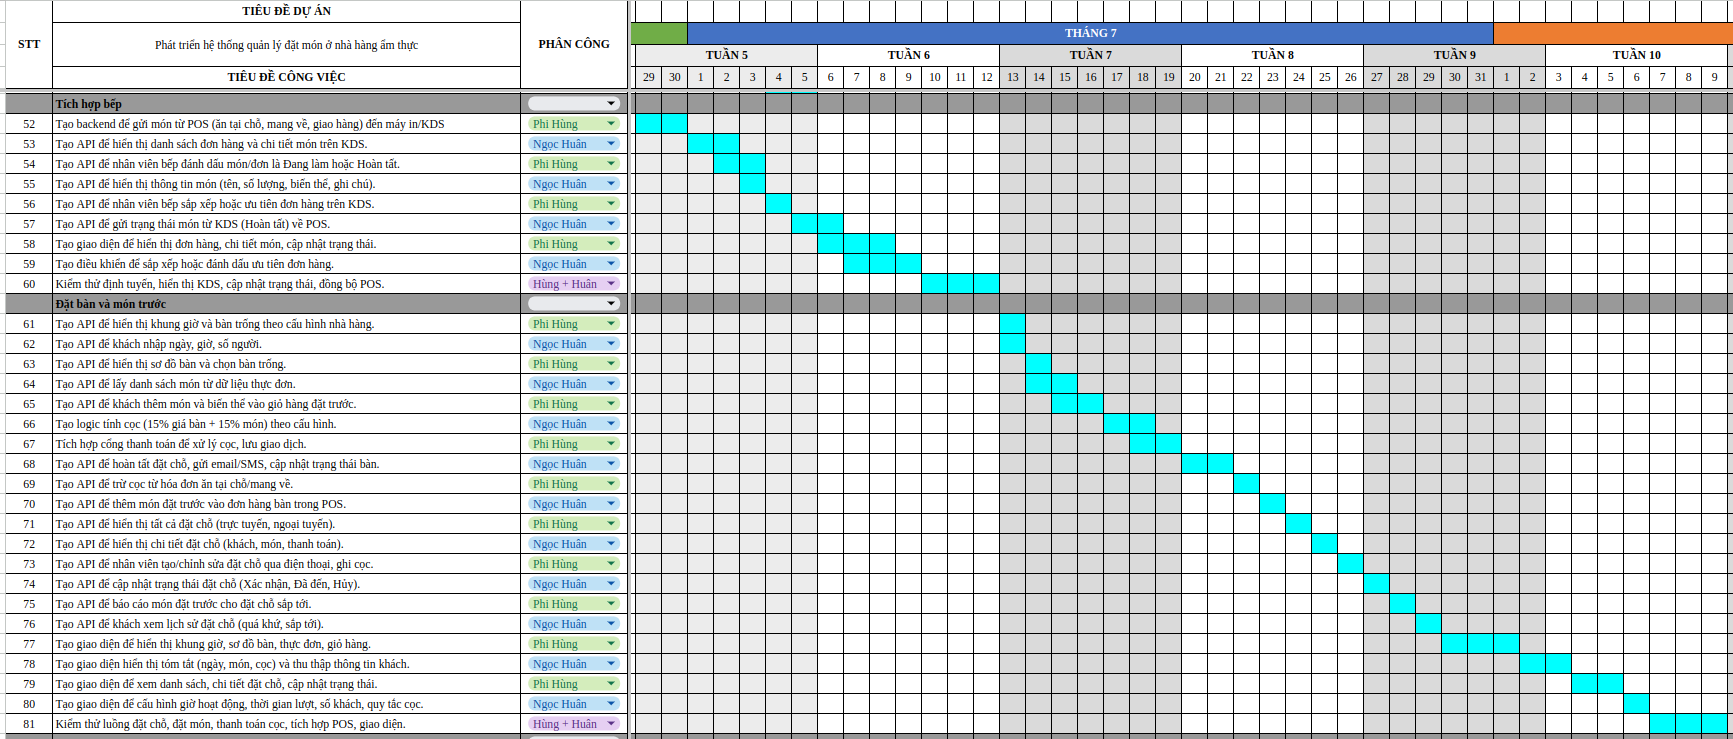
\includegraphics[width=\linewidth]{Images/gantt_3}
    \vspace{0.5cm}
    \caption{Biểu đồ Gantt cho các chức năng Tích hợp bếp và Đặt bàn/món trước}
    \label{fig:gantt_kitchen_booking}
\end{figure}

\begin{figure}[H]
    \centering
    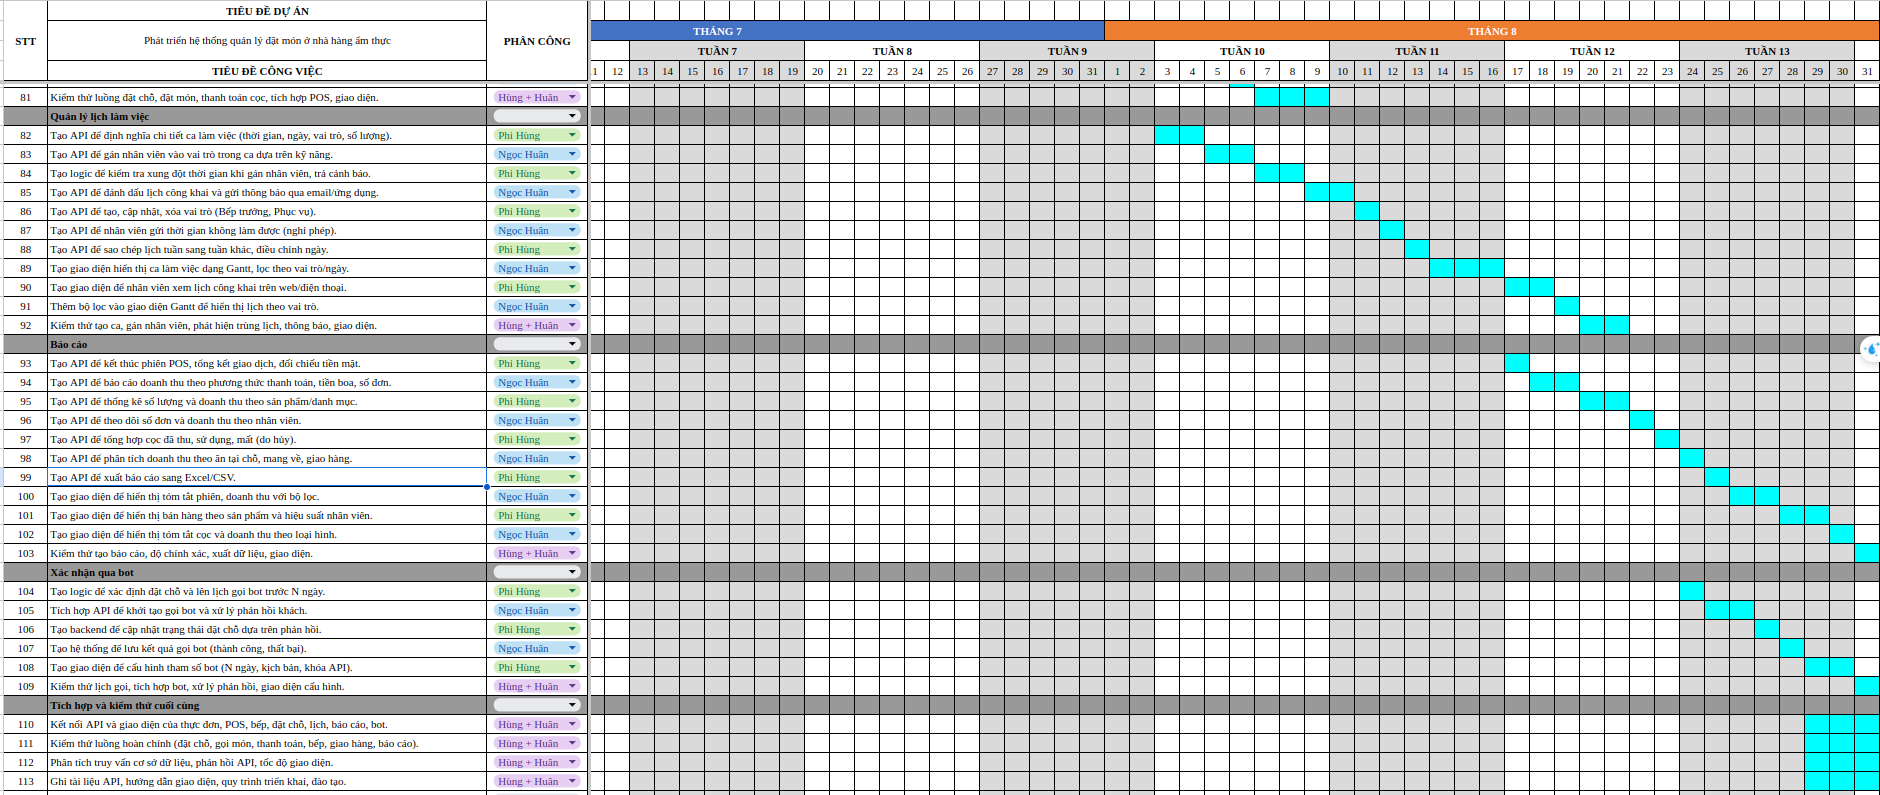
\includegraphics[width=\linewidth]{Images/gantt_4}
    \vspace{0.5cm}
    \caption{Biểu đồ Gantt cho các chức năng Quản lý lịch, Báo cáo, Xác nhận bot và Kiểm thử}
    \label{fig:gantt_schedule_report_test}
\end{figure}